\documentclass[11pt]{report}
\usepackage[abgabe]{protokoll}
\lstset{literate=
  {á}{{\'a}}1 {é}{{\'e}}1 {í}{{\'i}}1 {ó}{{\'o}}1 {ú}{{\'u}}1
  {Á}{{\'A}}1 {É}{{\'E}}1 {Í}{{\'I}}1 {Ó}{{\'O}}1 {Ú}{{\'U}}1
  {à}{{\`a}}1 {è}{{\`e}}1 {ì}{{\`i}}1 {ò}{{\`o}}1 {ù}{{\`u}}1
  {À}{{\`A}}1 {È}{{\'E}}1 {Ì}{{\`I}}1 {Ò}{{\`O}}1 {Ù}{{\`U}}1
  {ä}{{\"a}}1 {ë}{{\"e}}1 {ï}{{\"i}}1 {ö}{{\"o}}1 {ü}{{\"u}}1
  {Ä}{{\"A}}1 {Ë}{{\"E}}1 {Ï}{{\"I}}1 {Ö}{{\"O}}1 {Ü}{{\"U}}1
  {â}{{\^a}}1 {ê}{{\^e}}1 {î}{{\^i}}1 {ô}{{\^o}}1 {û}{{\^u}}1
  {Â}{{\^A}}1 {Ê}{{\^E}}1 {Î}{{\^I}}1 {Ô}{{\^O}}1 {Û}{{\^U}}1
  {œ}{{\oe}}1 {Œ}{{\OE}}1 {æ}{{\ae}}1 {Æ}{{\AE}}1 {ß}{{\ss}}1
  {ű}{{\H{u}}}1 {Ű}{{\H{U}}}1 {ő}{{\H{o}}}1 {Ő}{{\H{O}}}1  
  {ç}{{\c c}}1 {Ç}{{\c C}}1 {ø}{{\o}}1 {å}{{\r a}}1 {Å}{{\r A}}1
  {€}{{\EUR}}1 {£}{{\pounds}}1
}
\graphicspath{
  {pictures/}
}
\lstset{inputpath=source/}
\version{0.1$\alpha$}
\datum{\today}

%%
%% Titel, Autor und Betreuer
%%
\fachbereich{VII -- Elektrotechnik - Mechatronik - Optometrie --} 
\studiengang{Elektrotechnik - Schwerpunkt Elektronische Systeme}
\autor{Robby Kozok, Nic Frank Siebenborn, Pascal Kahlert}
\titel{Realisierung und Analyse des IIR-Filters} 
\untertitel{Laborbericht}
\modul{Digitale Signalverarbeitung III}
\betreuerFeld{
  \begin{tabular}{lr}
    \multicolumn{2}{l}{\textbf{Lehrkraft}}\\
    Prof.~Dr.-Ing~Marcus~Purat & Beuth Hochschule für Technik\\
  \end{tabular}
}
%%
%% Abkürzungen
%%
\makenoidxglossaries

\newacronym{fda}{FDA}{Filter Design and Analysis}





\begin{document}

\pagestyle{fancy}

%% Titelseite
\maketitle
\clearpage

%% Leerseite
\newpage

%\chapter*{Einleitung}

%% Einfügen des genutzten Aufgabenblattes. 
\clearpage
%% Seitenzahlen
\pagenumbering{roman}

%% Inhaltsverzeichnis
\tableofcontents

%% Abbildungsverzeichnis


%%Titelseite


\pagenumbering{arabic}


%%Kapitel
Die Aufgabe dieser �bung bestand darin, einen IIR Filter zu realisieren. Dabei sind folgende Pol- und Nullstellen vorgegeben:
    \centering
    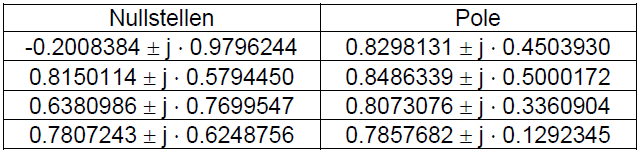
\includegraphics[width=\textwidth]{PolUndNullstellenIIR.png}
Diese haben wir zun\"achst in der z-Ebene gezeichnet, um die Pole und Nullstellen zu Teilsystemen zu kombinieren. 
Dabei waren die 3 Regeln aus der Aufgabenstellung zu beachten.
    \centering
    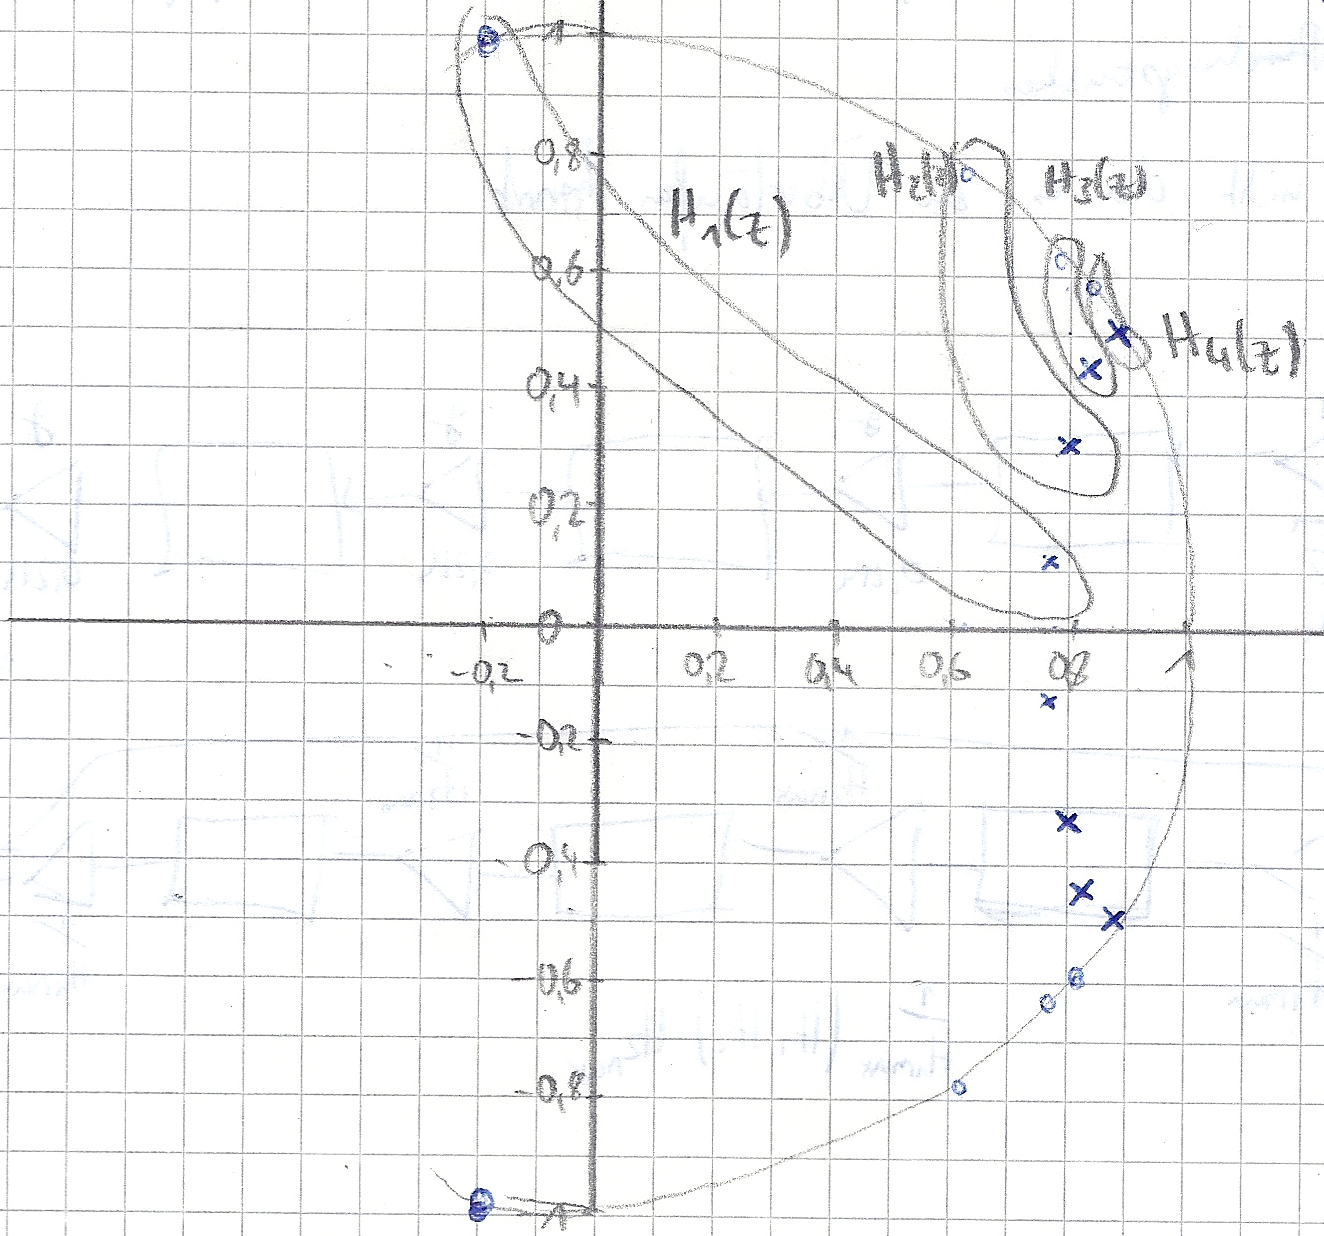
\includegraphics[width=\textwidth]{TeilsystemeZEbene.png}
    \caption{Kombinierte Pol- und Nullstellen}
    \label{fig:PolesAndZeros}
Nun haben wir die \"Ubertragungsfunktionen der 4 Teilsysteme aufgestellt in dem wir die kombinierten Pol- und Nullstellen in folgende Formel einsetzten.
    \centering
    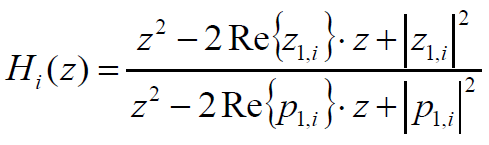
\includegraphics[width=\textwidth]{UeertragungsfunktionFormel.png}
Damit ergeben sich folgende \"Ubertragungsfunktionen:
\begin{equation}
  H_1(z)=\frac{1-1,6300228z^-1+1,00000009z^-2}{1-1,6972678z^-1+0,97019670z^-2}
  H_2(z)=\frac{1-1,5614486z^-1+0,99999995z^-2}{1-1,6596262z^-1+0,89144364z^-2}
  H_3(z)=\frac{1-1,2761982z^-1+1,00000006z^-2}{1-1,6146152z^-1+0,76470231z^-2}
  H_4(z)=\frac{1+0,4016768z^-1+1,00000003z^-2}{1-1,5715364z^-1+0,63413322z^-2}
\end{equation}

Nun war die Durchlassverst\"arkung des Gesamtsystems (ohne Verst\"rkungsfaktor g) f�r die Frequenz f=0 zu berechnen.
Bei einer Frequenz von 0Hz wird z zu 1. Damit lassen sich die Durchlassverst\"arkungen der Teilsysteme aussrechnen. Durch Multplikation dieser erhalten wir
die Durchlassverst\"arkung des Gesamtsystems.
\begin{equation}
  H_1(1)=1,3558
  H_2(1)=1,8921
  H_3(1)=4,8221
  H_4(1)=38,3655
  \Pi H_i(1)=38,3655*4,8221*1,8921*1,3558=474.5917
\end{equation}
Der Kehrwert der Gesamtverst\"arkung ergibt den Faktor mit dem das Gesamtsystem multipliziert werden muss damit die Durchlassverst\"arkung zu 1 wird.

\chapter{Realisierung des IIR-Filters}\label{Cha:RealIIR}
\section{Aufgabenstellung}
Die Aufgabe dieser Übung bestand darin, einen IIR Filter zu realisieren. Dabei galt besonderes Augenmerk der Minimierung von Rundungsfehlern sowie der Verhinderung von Überläufen.
\section{Durchf\"uhrung}
Das Filter wird auf die nachfolgenden vier Varianten implementiert. Vorab wurden dazu die Filterkoeffizienten entsprechend der Aufgabe nach aufsteigendem Radius im Einheitskreis sortiert.

Es wurden wie in der Aufgabe beschrieben die Dateien in ein neues Projekt eingefügt und wie im folgenden beschrieben entsprechend angepasst.
\subsection{Skalierung am Eingang}
Die einfachste Form der Skalierung ist die Skalierung am Eingang, wobei mit einem Divisor vor verwenden des Filters dividiert wird. Dazu wird zuerst die gesamte Verstärkung der Filter durch Multiplikation ermittelt.
Da es sich um einen Tiefpass handelt wird die Verstärkung bei 0Hz berechnet. Es folgt: z=1.
Gemäß folgender Formel ergibt sich eine Gesamtverstärkung von 474.5917.
\begin{equation}
\Pi H_i(1)=38,3655*4,8221*1,8921*1,3558=474.5917
\end{equation}
Daraus folgt die Anpassung der Datei process\textunderscore data.c wie folgt.\\

\begin{adjustbox}{width=\textwidth,height=\textheight,keepaspectratio}
 \begin{lstlisting}[title=processdata.c]{processdata.c}
// Definition der Filterkoeffizienten
#define BIQUAD_STAGES 4

// coef includes for all stages a scaling factor (2^s) and five coefficients
// in the order s, b2, b1, b0, a2, a1

// No scaling in stages (Low Pass)
const short coef[6*BIQUAD_STAGES] = {
	1, 16384, 6581	, 16384, -10390, 25748  //H4
	1, 16384, -20909, 16384, -12529, 26454, //H3
	1, 16384, -25583, 16384, -14605, 27191, //H2
	1, 16384, -26706, 16384, -15896, 27808, //H1
};

int iDelayline[2*BIQUAD_STAGES+2];	// delayline for left and right channel samples

IIRstateStereo iirLR={coef,iDelayline,BIQUAD_STAGES};

void process_data()
{
	//!! Scale before filtering
	sADC1L = sADC1L / 474.5917; //skalierungsfaktor aus Rechnung
	sADC1R = sADC1R / 474.5917;
	*(int*)(&sDAC1L) = iir_stereo(*(int*)(&sADC1L),&iirLR);

	//!! Scale after filtering
}

\end{lstlisting}
\end{adjustbox}
Die Interpretierung als 1.15 Format findet sich in den eingetragenen Koeffizienten nicht, sie wurden als short implementiert. Die Konvertierung erfolgte wie in früheren Laborübungen gesehen. Die Implementierung als short ermöglicht eine bessere Übersichtlichkeit und vermeidet Fehler. Die Zweite Anpassung war die eigentliche Skalierung am Eingang, hierzu wurde der zuvor ermittelte Divisor verwendet.\\
\begin{figure}[H]
  \centering
    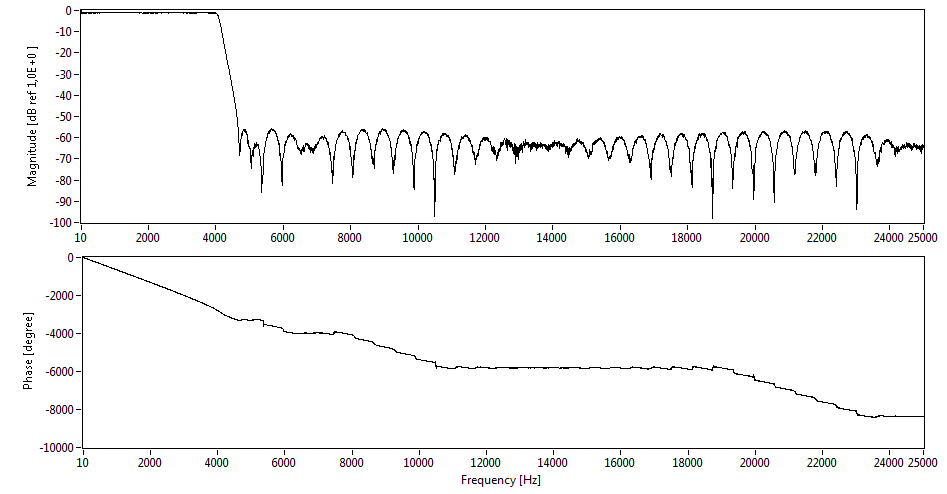
\includegraphics[width=\textwidth]{Freqgang3_1.png}
  \caption{Frequenzgang}
  \label{fig:Freqgang3_1}
\end{figure}
Hier wurde der Frequenzgang des Systems visualisiert, es ist deutlich das Tiefpassverhalten auszumachen. Die Grenzfrequenz liegt bei etwa 4kHz.\\
Zur weiteren Untersuchung wurde folgendes Sinussignal mit 2kHz Frequenz und 50mV Amplitude eingespeist.
\begin{figure}[H]
  \centering
    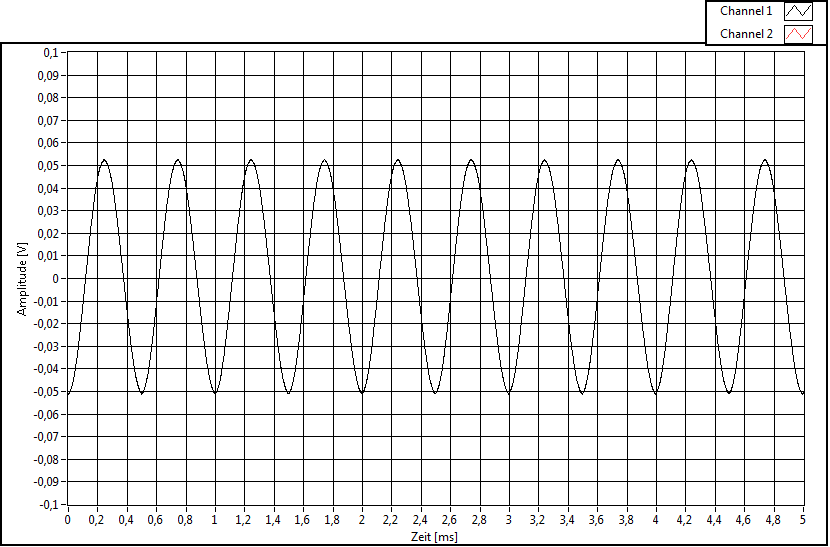
\includegraphics[width=\textwidth]{Eingangssignal50mv2kHz.png}
  \caption{Eingangssignal}
  \label{fig:Eingangssignal50mv2kHz}
\end{figure}
Wir haben am Eingang das nachfolgende Spektrum gemessen.
\begin{figure}[H]
  \centering
    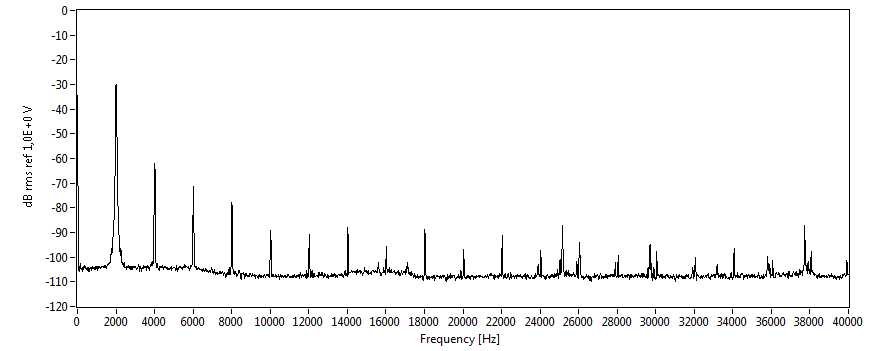
\includegraphics[width=\textwidth]{PowerspekEingang.png}
  \caption{Spektrum am Eingang}
  \label{fig:PowerspekEingang}
\end{figure}
Und am Ausgang hat man in nachstehendem Spektrum das Rauschen gut beobachten können.
\begin{figure}[H]
  \centering
    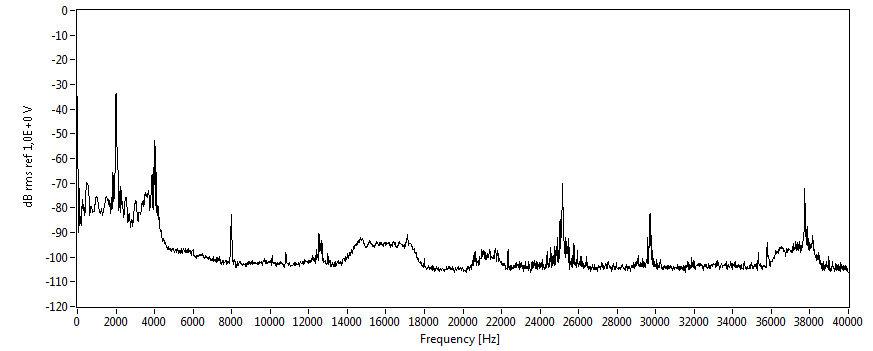
\includegraphics[width=\textwidth]{PowerspekAusgang.png}
  \caption{Spektrum am Ausgang}
  \label{fig:PowerspekAusgang}
\end{figure}
Es ist gut zu sehen, dass am Eingang mehrere Harmonische alle 2kHz zu sehen sind, umgeben von einem sehr geringen Rauschteppich bei unter -100dB. Am Ausgang hingegen ist das Tiefpassverhalten zu erkennen, was die erste Harmonische bei 4kHz (der Grenzfrequenz) noch leicht gedämpft darstellt, alle weiteren Harmonischen aber hinreichend unterdrückt. Außerdem lässt sich ein Rauschen ausmachen, was bis zur Grenzfrequenz um -80dB liegt. Dieses Bild entspricht unseren Erwartungen.
\subsection{Skalierung am Ausgang}
Entsprechend der Aufgabenstellung haben wir auch die Skalierung am Ausgang umgesetzt, wie erwartet übersteuerte das System massiv, was die Analyse der Implementierungsvariante unnütz machte. Aus diesem Grund verzichten wir wie Abgesprochen auf eine Auswertung an dieser Stelle.
\subsection{Gleichmäßige Skalierung}
Im dritten Teil der Übung wurde das Filter gleichmäßig über alle Teilfilter skaliert. Dazu wurde die Gesamtverstärkung aus dem ersten Teil gleichmäßig auf die Teilfilter aufgeteilt. Der Divisor ergibt sich also wie folgt:\\
\begin{equation}
\sqrt[4]{474.5917}=4,6675
\end{equation}
Bereits in der Vorbereitung wurden die Filterkoeffizienten durch diesen Quotienten geteilt und in das short Format gebracht. Somit ergibt sich folgende Änderung:\\
\begin{adjustbox}{width=\textwidth,height=\textheight,keepaspectratio}
 \begin{lstlisting}[title=processdata.c]
 
 // No scaling in stages (Low Pass)
const short coef[6*BIQUAD_STAGES] = {
	1, 3514, 1412, 3514, -2229, 5523, //H4
	1, 3514, -4485, 3514, -2687, 5674,//H3
	1, 3514, -5488, 3514, -3133, 5832,//H2
	1, 3514, -5728, 3514, -3410, 5965 //H1
};



int iDelayline[2*BIQUAD_STAGES+2];	// delayline for left and right channel samples

IIRstateStereo iirLR={coef,iDelayline,BIQUAD_STAGES};

void process_data()
{
	//!! Scale before filtering
	*(int*)(&sDAC1L) = iir_stereo(*(int*)(&sADC1L),&iirLR);
	//!! Scale after filtering

}

\end{lstlisting}
\end{adjustbox}
Es ist auch ersichtlich, dass die Skalierung am Ende im Gegensatz zur vorherigen Aufgabe entfernt wurde.\\
Bei dieser Art der Implementierung erwarten wir ab einer gewissen Amplitude Übersteuerungsfehler. So haben wir bei immer 2kHz verschiedene Amplituden auf das Signal gegeben und sind so sukzessive zu folgenden drei Bildern gelangt.
\begin{figure}[H]
  \centering
    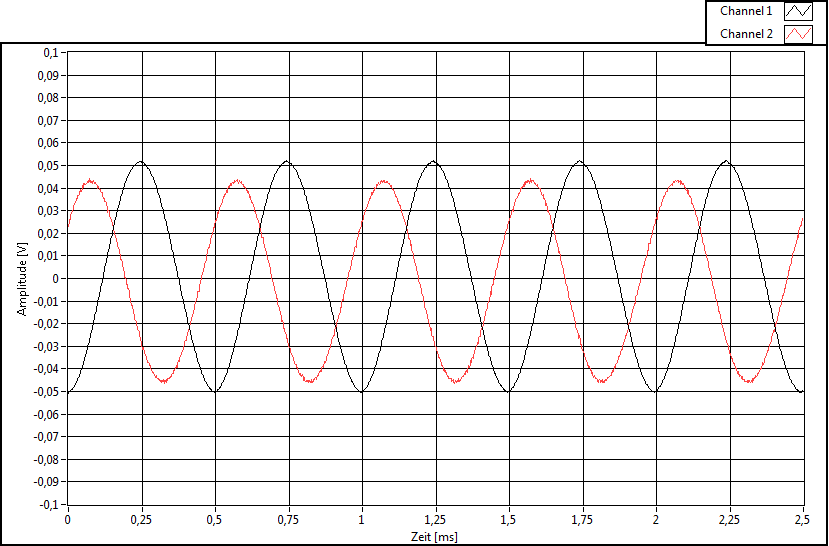
\includegraphics[width=\textwidth]{Sin50mV2kHz.png}
  \caption{50mV Amplitude}
  \label{fig:Sin50mV2kHz}
\end{figure}
\begin{figure}[H]
  \centering
    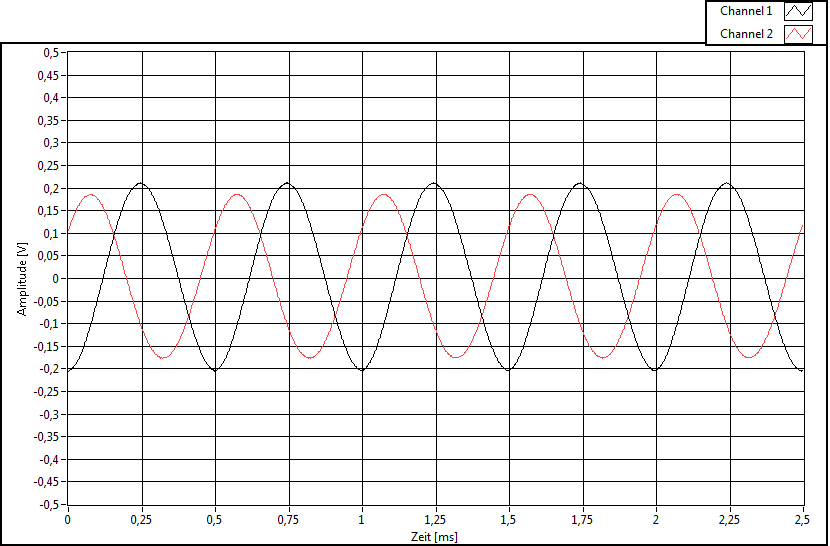
\includegraphics[width=\textwidth]{Sin200mV2kHz.png}
  \caption{200mV Amplitude}
  \label{fig:Sin200mV2kHz}
\end{figure}
\begin{figure}[H]
  \centering
    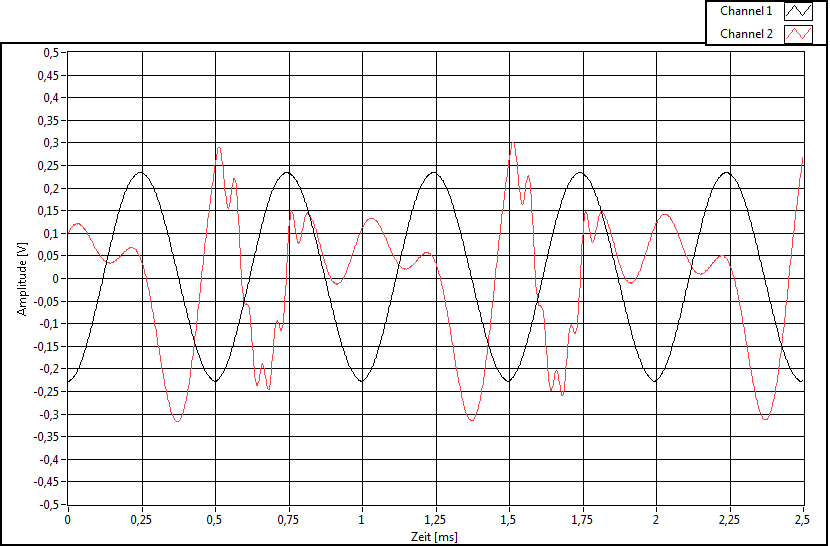
\includegraphics[width=\textwidth]{Sin230mV2kHz.png}
  \caption{230mV Amplitude}
  \label{fig:Sin230mV2kHz}
\end{figure}
Man sieht, dass das Ausgangssignal(rot) jeweils leicht gedämpft dem Eingangssignal entspricht außer bei 230mV Amplitude am Eingang. Der Erwartete Übersteuerungseffekt tritt also zwischen 200mV und 250mV auf. Dieses Ergebnis ist bei weitem besser als im Fall der Skalierung am Eingang.\\
Wir haben für die Fälle 50mV und 230mV die Spektren am Ausgang aufgenommen.\\
\begin{figure}[H]
  \centering
    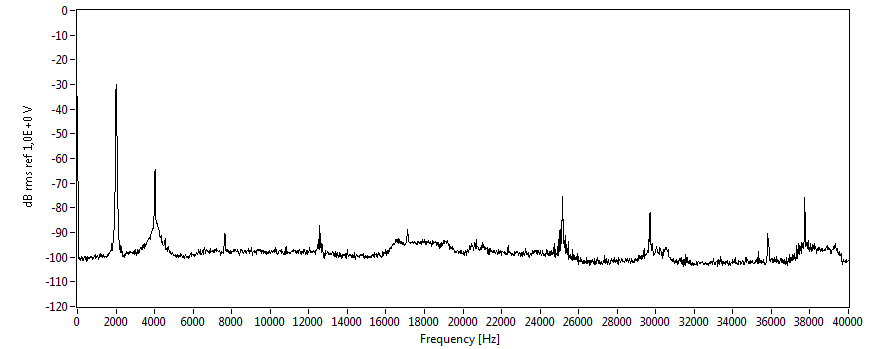
\includegraphics[width=\textwidth]{PowerSpektrumAusgang50mV2kHz.png}
  \caption{Spektrum am Ausgang 50mV}
  \label{fig:PowerSpektrumAusgang50mV2kHz}
\end{figure}
\begin{figure}[H]
  \centering
    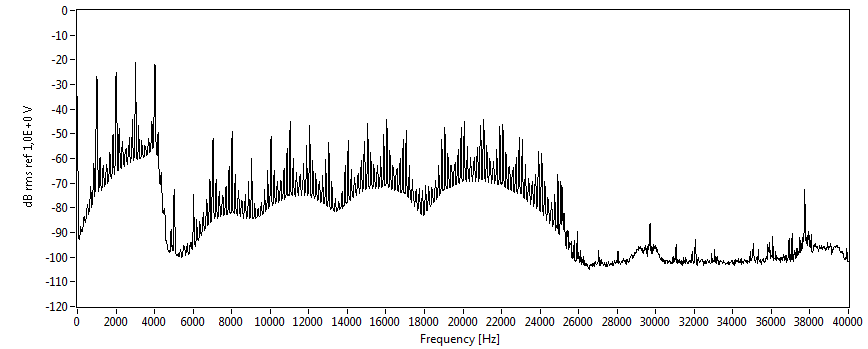
\includegraphics[width=\textwidth]{PowerSpektrumAusgang230mV2kHz.png}
  \caption{Spektrum am Ausgang 230mV}
  \label{fig:PowerSpektrumAusgang230mV2kHz}
\end{figure}
Bei dem Spektrum bei den 50mV ist das Ergebnis besser als bei der Skalierung am Eingang, so ist ein geringerer Rauschteppisch sowie eine Stärkere Unterdrückung der höheren Harmonischen zu erkennen. Die erste Harmonische ist wie erwartet leicht gedämpft gut erkennbar. Das Spektrum der Variante mit 230mV ist wie erwartet nicht sehr eindeutig. Mit Fantasie erkennt man ein Tiefpassverhalten mit einer Grenzfrequenz um 4kHz, weitere Deutung lässt die Abbildung nicht zu.

\subsection{Optimierte Skalierung}
Der letzte Optimierungsschritt ist die Skalierung an jedem Teilfilter opitmal passend zum Filter.
Dafür wurde folgendes Matlabfile erstellt.\\
\begin{adjustbox}{width=\textwidth,height=\textheight,keepaspectratio}
 \begin{lstlisting}[title=optimierung.m]
H1 = [-1 0 1 -0.9619429222893 1.847929303926];
H2 = [-1 0 1 -0.9633409060843 1.81768444585];
H3 = [-1 0 1 -0.9836465239584 1.819862361978];
H4 = [-1 0 1 -0.9850722601925 1.806715933748];

H=abs(freqz(H1(1:3),H1(4:5)));
g1=1/max(H);
H=g1*H;
H=H.*abs(freqz(H2(1:3),H2(4:5)));
g2=1/max(H);
H=g2*H;
H=H.*abs(freqz(H3(1:3),H3(4:5)));
g3=1/max(H);
H=g3*H;
H=H.*abs(freqz(H4(1:3),H4(4:5)));
g4=1/max(H);
H1n = (g1 .* H1(1:3) * 2^15)/2;
H2n = (g2 .* H2(1:3) * 2^15)/2;
H3n = (g3 .* H3(1:3) * 2^15)/2;
H4n = (g4 .* H4(1:3) * 2^15)/2;


\end{lstlisting}
\end{adjustbox}
Dieses Skript erstellt lediglich der Rechnung aus der Aufgabe entsprechend die einzelnen Skalierungsfaktoren und multipliziert diese mit den Filterkoeffizienten. Anschließend werden diese wieder in das handliche short Format gebracht.\\
Die neuen Filterkoeffizienten wurden daraufhin in das Programm gebracht.\\
\begin{adjustbox}{width=\textwidth,height=\textheight,keepaspectratio}
 \begin{lstlisting}[title=processdata.c]
const short coef[6*BIQUAD_STAGES] = {
	1,  427,    172,    427, -10390, 25748, //H4
	1, 3397,  -4336,   3397, -12529, 26454, //H3
	1, 9068, -14340,   9068, -14605, 27191, //H2
	1, 11981, -19529,  11981, -15896, 27808  //H1
};



int iDelayline[2*BIQUAD_STAGES+2];	// delayline for left and right channel samples

IIRstateStereo iirLR={coef,iDelayline,BIQUAD_STAGES};

void process_data()
{
	//!! Scale before filtering
	*(int*)(&sDAC1L) = iir_stereo(*(int*)(&sADC1L),&iirLR);
	//!! Scale after filtering

}
\end{lstlisting}
\end{adjustbox}
Man sieht, dass sich lediglich die Koeffizienten geändert haben und außerdem keinerlei Anpassung vorgenommen wurde.\\
Wir haben wie im Optimierungsfall zuvor die maximal mögliche Eingangsamplitude, die Fehlerfrei an den Ausgang gegeben wird ermittelt und visualisiert.
\begin{figure}[H]
  \centering
    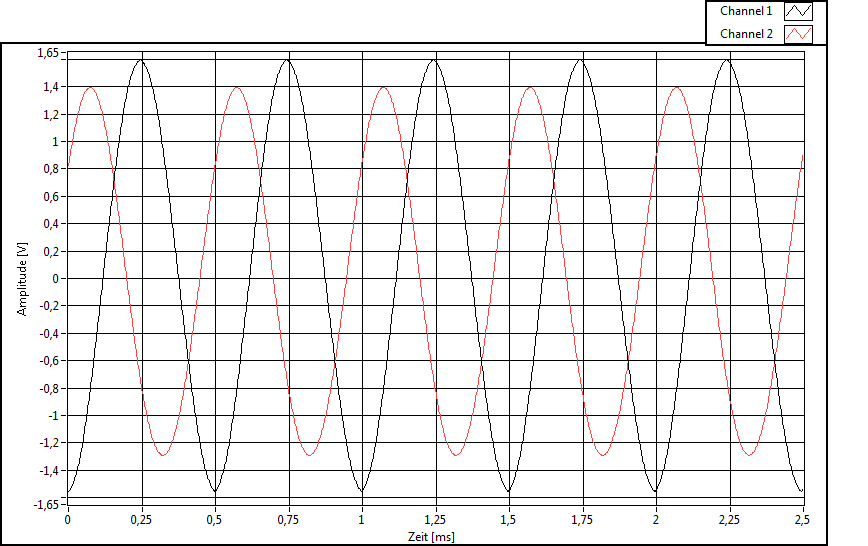
\includegraphics[width=\textwidth]{Sin1V61_2kHz.png}
  \caption{Sinus 1,61V}
  \label{fig:Sin1V61_2kHz}
\end{figure}
\begin{figure}[H]
  \centering
    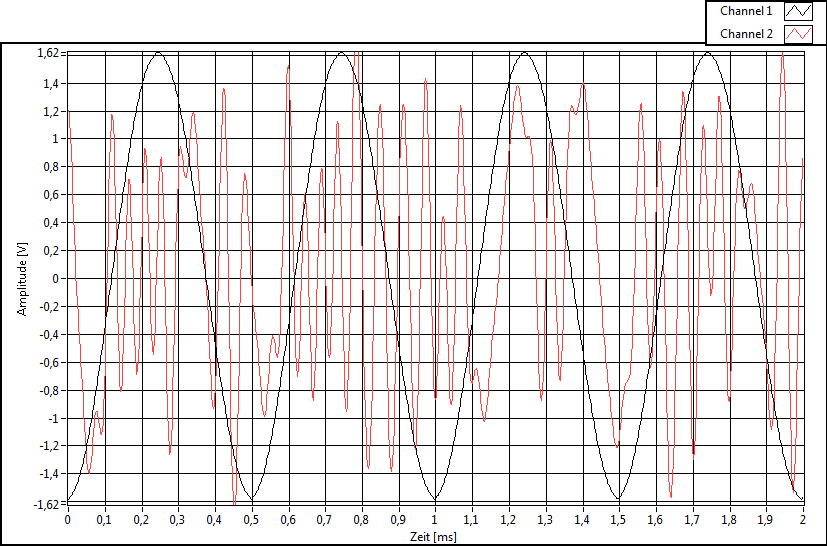
\includegraphics[width=\textwidth]{Sin1V62_2kHz.png}
  \caption{Sinus 1,62V}
  \label{fig:Sin1V62_2kHz}
\end{figure}
Es ist erkennbar, dass zwischen 1,61V und 1,62V Amplitude die Grenze liegt ab der der Fehler auftritt.
\begin{figure}[H]
  \centering
    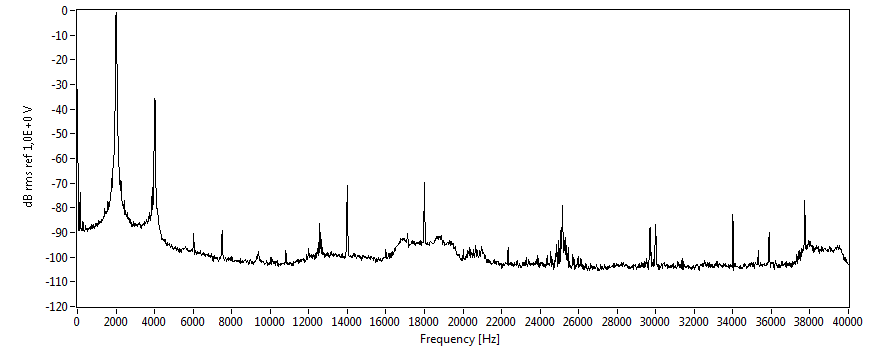
\includegraphics[width=\textwidth]{PowerSpektrumAusgang1V61_2kHz.png}
  \caption{Spektrum am Ausgang 1,61V}
  \label{fig:PowerSpektrumAusgang1V61_2kHz}
\end{figure}
\begin{figure}[H]
  \centering
    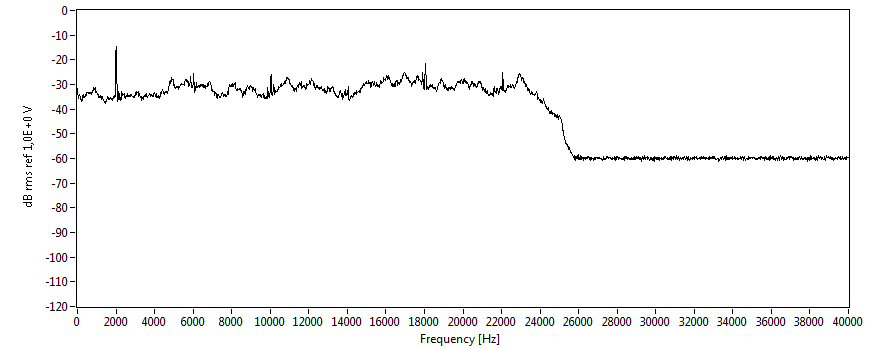
\includegraphics[width=\textwidth]{PowerSpektrumAusgang1V62_2kHz.png}
  \caption{Spektrum am Ausgang 1,62V}
  \label{fig:PowerSpektrumAusgang1V62_2kHz}
\end{figure}
Bei der Version mit 1,61V Amplitude ist der Peak bei 2kHz eindeutig zu erkennen, genau wie die erste Harmonische bei 4kHz, wie erwartet leicht gedämpft. Bei 1,62V Amplitude ist wie erwartet kein befriedigendes Ergebnis vorhanden, was bestätigt, dass die Grenzamplitude ab der das Übersteuern zwischen 1,61V und 1,62V liegt.\\ 
Als Resultat lässt sich festhalten, dass die letzte Variante der optimierten Anpassung zum Besten ergebnis führt, da hier die höchste Amplitude ohne Fehler auftritt. Diese Implementierung hat zwar den höchsten Implementierungsaufwand, aber keine Performancenachteile, da die Filterkoeffizienten hart gecodet wurden.

\chapter{Analyse des FIR-Filters}
\section{Aufgabenstellung}
In dieser Aufgabe sollte zunächst die 3dB-Grenzfrequenz des Tiefpass-Filters ermittelt werden.
Im weiteren Verlauf sollte mithilfe des \gls{fda} - Tools ein IIR-Bandpass-Filter entworfen werden.
Folgende Charakteristik ist dabei zu erreichen:
\begin{itemize}
\item Butterworth-Charakteristik
\item Stoppband-Frequenzen: 2000Hz, 4000Hz
\item Passband-Frequenzen: 2000Hz, 4000Hz
\item Passband-Welligkeit: 1dB
\item Stoppband-Dämpfung: 60dB
\end{itemize}
\section{Durchf\"uhrung}
\subsection*{IIR-Tiefpass-Filter}
Zur Ermittlung der 3dB-Grenzfrequenz sollte die Frequenz so eingestellt werden, dass das Ausgangssignal 70\% der Amplitude des Ausgangssignals bei 50Hz entspricht.
Dafür wurde die Amplitude bei 50Hz auf 1V eingestellt, danach haben wir uns das Spektrum des Systems angeschaut.\\\par Dies ist in Abbildung \ref{fig:SprektrumZoomSystem} zu sehen. Dort sehen wir 3dB-Dämpfung bei 4060Hz. Dies entspricht den Erwartungen, da der Filter seine Grenzfrequenz bei ungefähr 4kHz haben sollte. 
\begin{figure}[H]
  \centering
    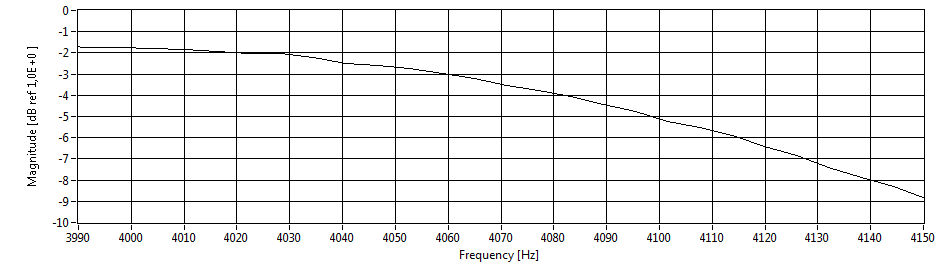
\includegraphics[width=\textwidth]{SpektrumEingezoomt.png}
  \caption{Ausschnitt des Spektrums des Systems}
  \label{fig:SprektrumZoomSystem}
\end{figure}


Im weiteren haben wir dann eine Aufnahme mit dem VI gemacht. Diese ist in Abbildung \ref{fig:4060HzScope} zu sehen, dieses Ergebnis war zu erwarten. Es ist zu sehen das das rote Ausgangssignal bei ungefähr 0,7V liegt und damit 70\% der ehemals 1V hat. Die Frequenz wurde auf 4060Hz eingestellt.
\begin{figure}[H]
  \centering
    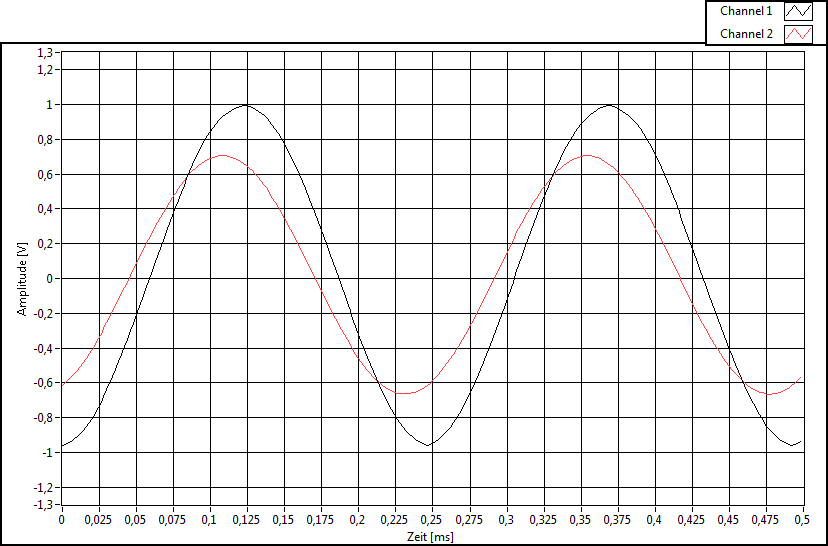
\includegraphics[width=\textwidth]{Sin1V_4,060kHz.png}
  \caption{Ein- und Ausgangssignal nebeneinander}
  \label{fig:4060HzScope}
\end{figure}

\subsection*{IIR-Bandpass-Filter}
Der zweite Teil behandelte die Erstellung IIR-Bandpass-Filters. Zu allererst mussten dafür die Koeffizienten generiert werden. Diese wurde dann mit Matlab abermals optimiert.
\lstinputlisting[title=Matlab-Code zur Optimierung der Koeffizienten]{OptimierungBandpass.m}

Die Berechnung erfolgte wie bereits für den Tiefpass-Filter. Anschließend mussten die Koeffizienten in den C-Code eingefügt werden.\\
\begin{adjustbox}{width=\textwidth, keepaspectratio} 
  \label{code:procdataKompFIR}
  \begin{lstlisting}[title=Codeausschnitt der modifizierten process\_data.c]
// Definition der Filterkoeffizienten
#define BIQUAD_STAGES 4 // Anzahl der Koeffizienten

const short coef[6*BIQUAD_STAGES] = {
	1,  -122,	   0,	 122, -16139, 30276, //H4
	1,  -651,      0,	 651, -16116, 29781, //H3
	1,  -343,      0,	 343, -15783, 29817, //H2
	1,  -451,	   0,	 451, -15760, 29601  //H1
};
  \end{lstlisting}
\end{adjustbox}

Zur Überprüfung der Implementierung wurde der Amplitudengang und die Sprungantwort aufgenommen. Diese wurden dann mit den von Matlab generierten Idealen Vorgaben verglichen.
\begin{figure}[H]
  \centering
    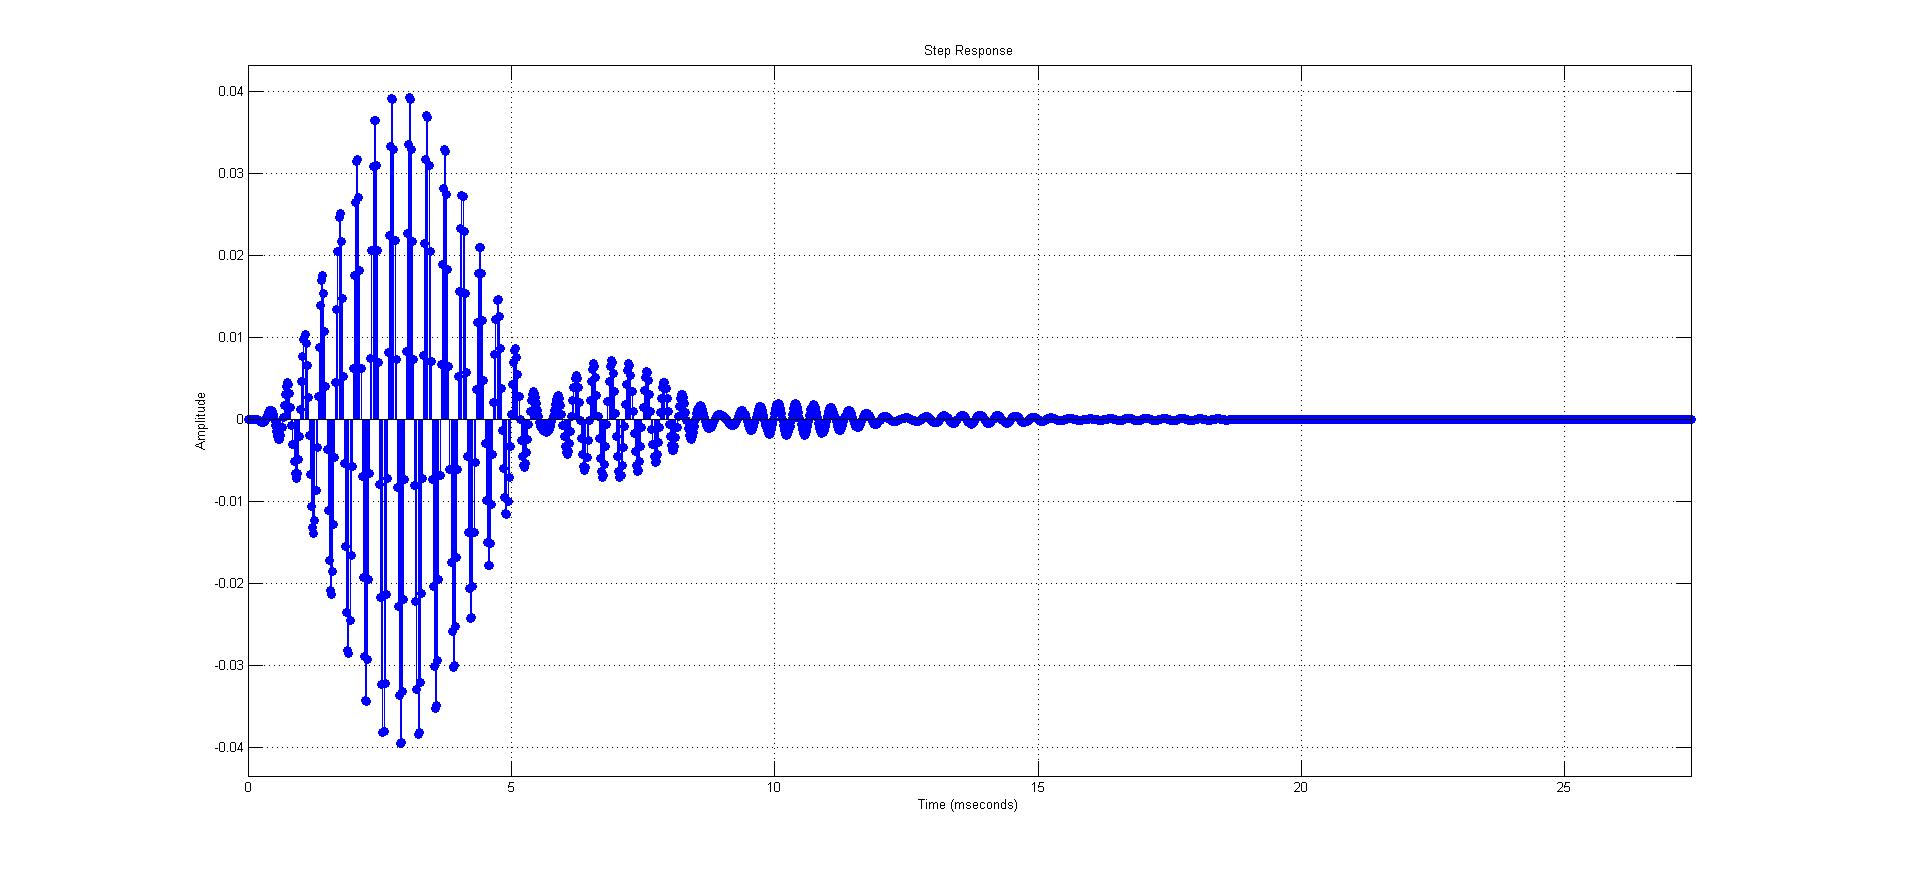
\includegraphics[width=\textwidth]{SprungantwortIdeal.png}
  \caption{Ideale Sprungantwort des Filters}
  \label{fig:SprungBandIdeal}
\end{figure}
\begin{figure}[H]
  \centering
    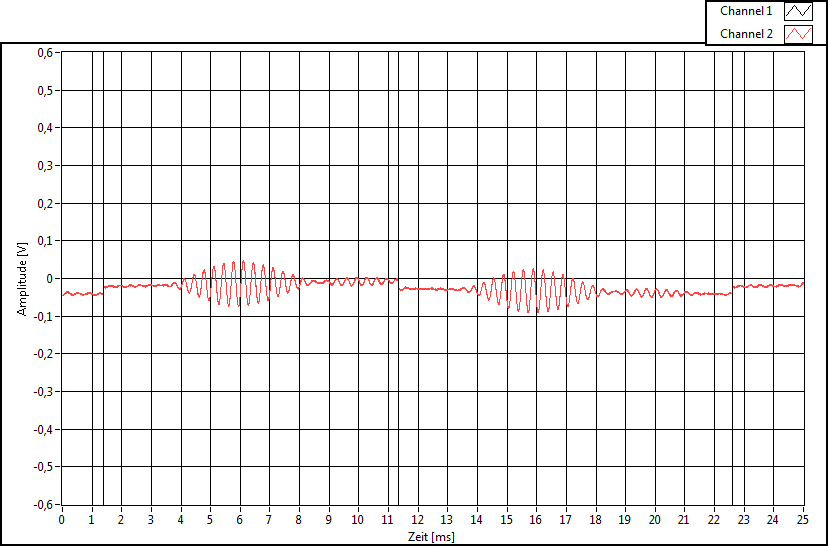
\includegraphics[width=\textwidth]{SprungantwortZoomReal.png}
  \caption{Reale Sprungantwort des Filters}
  \label{fig:SprungBandReal}
\end{figure}

In Abbildung \ref{fig:SprungBandIdeal} ist die Ideale Sprungantwort und in Abbildung \ref{fig:SprungBandReal} die Reale Sprungantwort des Filters zu sehen.
Beide Sprungantworten gleichen sich weites gehend. Die Amplituden der beiden Sprungantworten unterscheiden sich leicht, denn der reale Sprung ist bei uns ein Rechteck, welches eine Amplitude von \begin{math} V_{pp} = 2V \end{math} hat wohingegen der ideale Sprung nur eine Amplitude von \begin{math} V_{pp} = 1V \end{math} besitzt. Dies erklärt die leicht kleinere Amplitude der idealen Sprungantwort.\\ Ein weiterer Unterschied, ist die leichte Dämpfung auf dem Gleichspannungsanteil. Dies erklärt sich durch die Dämpfung des Systems.

\begin{figure}[H]
  \centering
    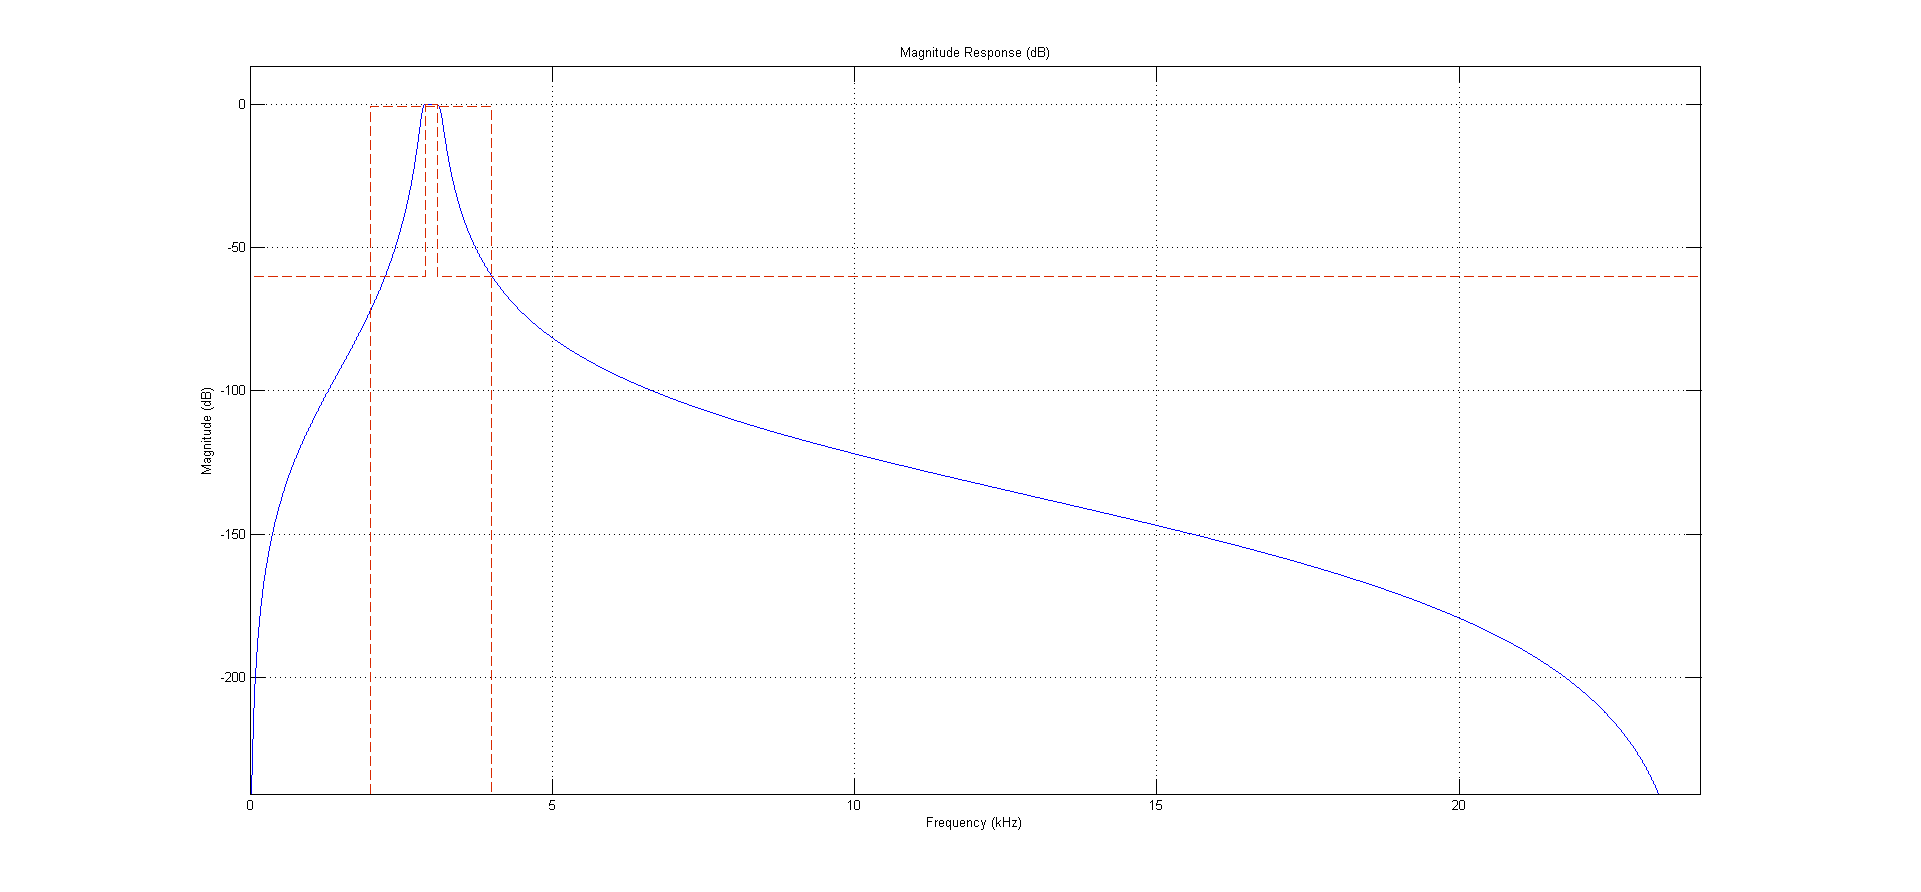
\includegraphics[width=\textwidth]{AmplitudengangIdeal.png}
  \caption{Idealer Amplitudengang des Filters}
  \label{fig:AmpBandIdeal}
\end{figure}
\begin{figure}[H]
  \centering
    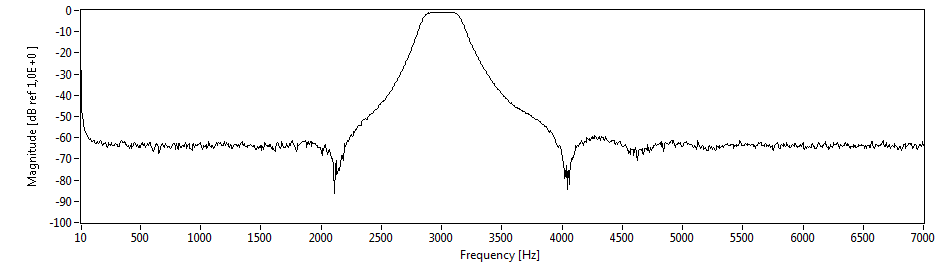
\includegraphics[width=\textwidth]{AmplitudengangReal.png}
  \caption{Realer Amplitudengang des Filters}
  \label{fig:AmpBandReal}
\end{figure}

Abbildung \ref{fig:AmpBandIdeal} ist der ideale Amplitudengang und in Abbildung \ref{fig:AmpBandReal} der reale Amplitudengang zu sehen. 
Beide Amplitudengänge sind sich ähnlich, weisen allerdings im Detail gravierende Unterschiede auf.
So erreicht der Reale Filter kein 0dB Dämpfung an der Passfrequenz sondern hat eine Dämpfung von 1dB, dies ist die Dämpfung des Systems. Außerdem wird in den Stoppbändern keine Dauerhafte Dämpfung von unter 60dB erreicht. Dies liegt ebenfalls am System, da dieses 10 Bit nutzt und dabei
0 dB bis -60 dB bei einer Auflösung von 1 dB darstellt. Allerdings erfüllt dies trotzdem die Anforderung. \todo{Negative Peaks erklrären}


%%Anhang
\begin{appendix}
  \chapter{Quelltext-Dateien}




\end{appendix}

\clearpage\newpage
\listoffigures

\printnoidxglossary[type=\acronymtype,title=Abkürzungsverzeichnis]

\end{document}